%%%%%%%%%%%%%%%%%%%%%%%%%%%%%%%%%%%%%%%%%
% Masters/Doctoral Thesis 
% LaTeX Template
% Version 2.5 (27/8/17)
%
% This template was downloaded from:
% http://www.LaTeXTemplates.com
%
% Version 2.x major modifications by:
% Vel (vel@latextemplates.com)
%
% This template is based on a template by:
% Steve Gunn (http://users.ecs.soton.ac.uk/srg/softwaretools/document/templates/)
% Sunil Patel (http://www.sunilpatel.co.uk/thesis-template/)
%
% Template license:
% CC BY-NC-SA 3.0 (http://creativecommons.org/licenses/by-nc-sa/3.0/)
%
%%%%%%%%%%%%%%%%%%%%%%%%%%%%%%%%%%%%%%%%%

%----------------------------------------------------------------------------------------
%	PACKAGES AND OTHER DOCUMENT CONFIGURATIONS
%----------------------------------------------------------------------------------------

\documentclass[
11pt, % The default document font size, options: 10pt, 11pt, 12pt
%oneside, % Two side (alternating margins) for binding by default, uncomment to switch to one side
english, % ngerman for German
singlespacing, % Single line spacing, alternatives: onehalfspacing or doublespacing
%draft, % Uncomment to enable draft mode (no pictures, no links, overfull hboxes indicated)
%nolistspacing, % If the document is onehalfspacing or doublespacing, uncomment this to set spacing in lists to single
%liststotoc, % Uncomment to add the list of figures/tables/etc to the table of contents
%toctotoc, % Uncomment to add the main table of contents to the table of contents
%parskip, % Uncomment to add space between paragraphs
%nohyperref, % Uncomment to not load the hyperref package
headsepline, % Uncomment to get a line under the header
%chapterinoneline, % Uncomment to place the chapter title next to the number on one line
%consistentlayout, % Uncomment to change the layout of the declaration, abstract and acknowledgements pages to match the default layout
]{MastersDoctoralThesis} % The class file specifying the document structure

\usepackage[utf8]{inputenc} % Required for inputting international characters
\usepackage[T1]{fontenc} % Output font encoding for international characters

\usepackage{mathpazo} % Use the Palatino font by default

\usepackage[backend=bibtex,style=authoryear,natbib=true]{biblatex} % Use the bibtex backend with the authoryear citation style (which resembles APA)

\addbibresource{example.bib} % The filename of the bibliography

\usepackage[autostyle=true]{csquotes} % Required to generate language-dependent quotes in the bibliography

%----------------------------------------------------------------------------------------
%	MARGIN SETTINGS
%----------------------------------------------------------------------------------------

\geometry{
	paper=a4paper, % Change to letterpaper for US letter
	inner=2.5cm, % Inner margin
	outer=3.8cm, % Outer margin
	bindingoffset=.5cm, % Binding offset
	top=1.5cm, % Top margin
	bottom=1.5cm, % Bottom margin
	%showframe, % Uncomment to show how the type block is set on the page
}

%----------------------------------------------------------------------------------------
%	THESIS INFORMATION
%----------------------------------------------------------------------------------------

\thesistitle{Thesis Title} % Your thesis title, this is used in the title and abstract, print it elsewhere with \ttitle
\supervisor{Dr. James \textsc{Smith}} % Your supervisor's name, this is used in the title page, print it elsewhere with \supname
\examiner{} % Your examiner's name, this is not currently used anywhere in the template, print it elsewhere with \examname
\degree{Doctor of Philosophy} % Your degree name, this is used in the title page and abstract, print it elsewhere with \degreename
\author{John \textsc{Smith}} % Your name, this is used in the title page and abstract, print it elsewhere with \authorname
\addresses{} % Your address, this is not currently used anywhere in the template, print it elsewhere with \addressname

\subject{Biological Sciences} % Your subject area, this is not currently used anywhere in the template, print it elsewhere with \subjectname
\keywords{} % Keywords for your thesis, this is not currently used anywhere in the template, print it elsewhere with \keywordnames
\university{\href{http://www.university.com}{University Name}} % Your university's name and URL, this is used in the title page and abstract, print it elsewhere with \univname
\department{\href{http://department.university.com}{Department or School Name}} % Your department's name and URL, this is used in the title page and abstract, print it elsewhere with \deptname
\group{\href{http://researchgroup.university.com}{Research Group Name}} % Your research group's name and URL, this is used in the title page, print it elsewhere with \groupname
\faculty{\href{http://faculty.university.com}{Faculty Name}} % Your faculty's name and URL, this is used in the title page and abstract, print it elsewhere with \facname

\AtBeginDocument{
\hypersetup{pdftitle=\ttitle} % Set the PDF's title to your title
\hypersetup{pdfauthor=\authorname} % Set the PDF's author to your name
\hypersetup{pdfkeywords=\keywordnames} % Set the PDF's keywords to your keywords
}

\begin{document}

\frontmatter % Use roman page numbering style (i, ii, iii, iv...) for the pre-content pages

\pagestyle{plain} % Default to the plain heading style until the thesis style is called for the body content

%----------------------------------------------------------------------------------------
%	TITLE PAGE
%----------------------------------------------------------------------------------------

\begin{titlepage}
\begin{center}

\vspace*{.06\textheight}
{\scshape\LARGE \univname\par}\vspace{1.5cm} % University name
\textsc{\Large Doctoral Thesis}\\[0.5cm] % Thesis type

\HRule \\[0.4cm] % Horizontal line
{\huge \bfseries \ttitle\par}\vspace{0.4cm} % Thesis title
\HRule \\[1.5cm] % Horizontal line
 
\begin{minipage}[t]{0.4\textwidth}
\begin{flushleft} \large
\emph{Author:}\\
\href{http://www.johnsmith.com}{\authorname} % Author name - remove the \href bracket to remove the link
\end{flushleft}
\end{minipage}
\begin{minipage}[t]{0.4\textwidth}
\begin{flushright} \large
\emph{Supervisor:} \\
\href{http://www.jamessmith.com}{\supname} % Supervisor name - remove the \href bracket to remove the link  
\end{flushright}
\end{minipage}\\[3cm]
 
\vfill

\large \textit{A thesis submitted in fulfillment of the requirements\\ for the degree of \degreename}\\[0.3cm] % University requirement text
\textit{in the}\\[0.4cm]
\groupname\\\deptname\\[2cm] % Research group name and department name
 
\vfill

{\large \today}\\[4cm] % Date
%\includegraphics{Logo} % University/department logo - uncomment to place it
 
\vfill
\end{center}
\end{titlepage}

%----------------------------------------------------------------------------------------
%	DECLARATION PAGE
%----------------------------------------------------------------------------------------

\begin{declaration}
\addchaptertocentry{\authorshipname} % Add the declaration to the table of contents
\noindent I, \authorname, declare that this thesis titled, \enquote{\ttitle} and the work presented in it are my own. I confirm that:

\begin{itemize} 
\item This work was done wholly or mainly while in candidature for a research degree at this University.
\item Where any part of this thesis has previously been submitted for a degree or any other qualification at this University or any other institution, this has been clearly stated.
\item Where I have consulted the published work of others, this is always clearly attributed.
\item Where I have quoted from the work of others, the source is always given. With the exception of such quotations, this thesis is entirely my own work.
\item I have acknowledged all main sources of help.
\item Where the thesis is based on work done by myself jointly with others, I have made clear exactly what was done by others and what I have contributed myself.\\
\end{itemize}
 
\noindent Signed:\\
\rule[0.5em]{25em}{0.5pt} % This prints a line for the signature
 
\noindent Date:\\
\rule[0.5em]{25em}{0.5pt} % This prints a line to write the date
\end{declaration}

\cleardoublepage

%----------------------------------------------------------------------------------------
%	QUOTATION PAGE
%----------------------------------------------------------------------------------------

\vspace*{0.2\textheight}

\noindent\enquote{\itshape Thanks to my solid academic training, today I can write hundreds of words on virtually any topic without possessing a shred of information, which is how I got a good job in journalism.}\bigbreak

\hfill Dave Barry

%----------------------------------------------------------------------------------------
%	ABSTRACT PAGE
%----------------------------------------------------------------------------------------

\begin{abstract}
\addchaptertocentry{\abstractname} % Add the abstract to the table of contents
The Thesis Abstract is written here (and usually kept to just this page). The page is kept centered vertically so can expand into the blank space above the title too\ldots
\end{abstract}

%----------------------------------------------------------------------------------------
%	ACKNOWLEDGEMENTS
%----------------------------------------------------------------------------------------

\begin{acknowledgements}
\addchaptertocentry{\acknowledgementname} % Add the acknowledgements to the table of contents
The acknowledgments and the people to thank go here, don't forget to include your project advisor\ldots
\end{acknowledgements}

%----------------------------------------------------------------------------------------
%	LIST OF CONTENTS/FIGURES/TABLES PAGES
%----------------------------------------------------------------------------------------

\tableofcontents % Prints the main table of contents

\listoffigures % Prints the list of figures

\listoftables % Prints the list of tables

%----------------------------------------------------------------------------------------
%	ABBREVIATIONS
%----------------------------------------------------------------------------------------

\begin{abbreviations}{ll} % Include a list of abbreviations (a table of two columns)

\textbf{LAH} & \textbf{L}ist \textbf{A}bbreviations \textbf{H}ere\\
\textbf{WSF} & \textbf{W}hat (it) \textbf{S}tands \textbf{F}or\\

\end{abbreviations}

%----------------------------------------------------------------------------------------
%	PHYSICAL CONSTANTS/OTHER DEFINITIONS
%----------------------------------------------------------------------------------------

\begin{constants}{lr@{${}={}$}l} % The list of physical constants is a three column table

% The \SI{}{} command is provided by the siunitx package, see its documentation for instructions on how to use it

Speed of Light & $c_{0}$ & \SI{2.99792458e8}{\meter\per\second} (exact)\\
%Constant Name & $Symbol$ & $Constant Value$ with units\\

\end{constants}

%----------------------------------------------------------------------------------------
%	SYMBOLS
%----------------------------------------------------------------------------------------

\begin{symbols}{lll} % Include a list of Symbols (a three column table)

$a$ & distance & \si{\meter} \\
$P$ & power & \si{\watt} (\si{\joule\per\second}) \\
%Symbol & Name & Unit \\

\addlinespace % Gap to separate the Roman symbols from the Greek

$\omega$ & angular frequency & \si{\radian} \\

\end{symbols}

%----------------------------------------------------------------------------------------
%	DEDICATION
%----------------------------------------------------------------------------------------

\dedicatory{For/Dedicated to/To my\ldots} 

%----------------------------------------------------------------------------------------
%	THESIS CONTENT - CHAPTERS
%----------------------------------------------------------------------------------------

\mainmatter % Begin numeric (1,2,3...) page numbering

\pagestyle{thesis} % Return the page headers back to the "thesis" style

% Include the chapters of the thesis as separate files from the Chapters folder
% Uncomment the lines as you write the chapters

\chapter{Introduccion}

\label{Chapter1}

En este capitulo se muestra la principal motivacion para el desarrollo de esta tesis, 
asi como una breve perspectiva de la problematica general. Como capitulo introductorio este contiene la introduccion,
el planteamiento del problema, el objetivo, las fronteras del estudio y la estructura del escrito.

\section{Introduccion}

En el area de la fisica de altas energias (HEP) las tecnicas de aprendizaje maquina (ML) siempre estuvieron presentes. 
Debido a la sorprendente efectividad de tecnicas modernas como el aprendizaje profundo, 
se comenzaron a adaptar y desarrollar estos metodos en todos los rubros del campo. 
Algunas de las aplicaciones van desde los enfoques que se tienen en la parte experimental, la fenomenologica o en el anlisis teorico de los eventos.

En los experimentos mas importantes del campo, el tratamiento y analisis de datos es una tarea fundamental.
Tecnicas como arboles de desicion, maquinas de soporte vectorial, algoritmos geneticos, entre otras, 
fallaban cuando la dimensionalidad de los datos aumentaba.
Como referencia de la alta dimensionalidad, en el gran colisionador de hadrones LHC, las colisiones ocurren con una frecuencia de aproximadamente 40Mhz,
ademas de que cada colision genera un gran numero de particulas y en particular el LHC tiene alrededor $O(10^8)$ sensores para su deteccion.

Debido a que las observaciones son fundamentalmente probabilisticas se tiene un modelo 
estadistico que describe la probabilidad de observar un evento dado los parametros de una teoria.
Pero la alta dimensionalidad, junto con los grandes volumenes de datos generan un problema, ya que el 
modelo de los datos experimentales no se conoce explicitamente.
Sin embargo, si se tiene acceso a muestras de datos generados por simuladores estocasticos que modelan la fisica de las interacciones.
Herramientas como PYTHIA, HERWING, GEANT, CORSIKA se les suele denominar como simuladores de Monte Carlo, los cuales cumplen  con dos necesidades,
la primera es aproximar el modelo estadistico al muestrar de un espacio enorme de procesos no observados o latentes y la segunda es generar una base de datos.

Entre las tareas de bajo nivel se tiene la identificacion de particulas y la reconstruccion de la energia/momento de la particula en cuestion.
Debido a que los simuladores completos que describen las interacciones de las particulas con la materia, son computacionalmente intensos
y se llevan gran parte del presupuesto computacional de las colaboraciones, los simuladores rapidos son escenciales.
Simuladores como GEANT y CORSIKA que generan una excelente descripcion de interacciones hadronicas son lentos.
En los ultimos anos ha nacido un gran interes por usar redes neuronales generativas para aumentar la velocidad de las simulaciones y tal vez
llegar a usar estos metodos directamente en datos generados por colisiones reales y hacer tunning en en el momento.

El presente trabajo esta fundamentado en el desarrollo de algoritmos de aprendizaje maquina profundo, especificamente reges generativas GAN 
para la generacion de interacciones hadronicas. Esto debido a la necesidad de generar simulaciones precisas y de una manera mas rapida,
ya que actualizaciones a dichos experimentos como el de Alta Luminosidad al LHC exigiran una mayor capacidad computacional que no se tiene con la proyeccion de presupuestos actuales.
Existe un gran interes por parte de la comunidad en usar metodos de aprendizaje no supervisado como GANs o VAEs para generar espacios de caracteristicas con una dimensionalidad alta.
Uno de los mayores desafios que hay al usar estos metodos es como cuantificar su desempeno.

\section{Plantamiento del problema}

El planteamineto se fundamenta en lo siguiente:

\emph{Sera posible disenar un metodo que utilize redes neuronales generativas que logre simular cascadas hadronicas precisas y a su vez la aquitectura no mezcle sus paramatros latentes que podrian estar asociados a la energia y momento de la particula.} 


\section{Objetivo de la tesis}
Objetivo principal:
\begin{itemize}
    \item Disenar y implementar una red neuronal generativa que no mezcle sus parametros latentes para generar cascadas hadornicas acordes a simulaciones obtenidas por el software CORSIKA. 
\end{itemize}

Objetivos particulares:
\renewcommand{\theenumi}{\roman{enumi}}%
\begin{enumerate}
    \item Disenar una arquitectura que integre algunos metodos de aprendizaje no supervisado para la simulacion de interacciones hadronicas.
    \item Entrenar esa arquitectura con una base de datos generada medienta el software CORSIKA.
    \item Mostrar el algoritmo que genera las simulaciones y comparar con simulaciones generadas mediante CORSIKA.
\end{enumerate}

\section{Delimitacion del tema}


\section{Contribucion de la tesis}


\section{Organizacion de la tesis}

%% Chapter Template

\chapter{Estado del arte} % Main chapter title

\label{Chapter2} % Change X to a consecutive number; for referencing this chapter elsewhere, use \ref{ChapterX}

%----------------------------------------------------------------------------------------
%	SECTION 1
%----------------------------------------------------------------------------------------
El presente capítulo proporciona el estado del arte mediante la revisión de conceptos y trabajos referentes a cascadas atmosféricas, detectores de partículas, simuladores y modelos generativos para establecer el fundamento del desarrollo de este trabajo. 

\section{Antecedentes}

El problema de reducir el costo computacional que experimentos en la física de altas energías (HEP) dedican a simulaciones ha tenido mucha atención en los últimos años, tanto que estudiar técnicas de aprendizaje máquina aplicadas al campo, se incluyeron como un área estratégica de inversiones iniciales para enfrentar los desafíos que actualizaciones como HL-LHC presentarán en los próximos años. 

El aprendizaje máquina siempre ha estado presente en los flujos de trabajo de experimentos en HEP, sin embargo técnicas modernas del aprendizaje profundo han comenzado a introducirse a procesos de análisis. En específico se ha visto que los modelos generativos permiten acelerar los tiempos de generación de simulaciones, debido a lo anterior es de suma importancia estudiar estas técnicas para que así puedan ser agregadas a próximas versiones de simuladores como GEANTV, CORSIKA8, etc.

Algunos investigadores que usan modelos generativos para acelerar simulaciones son Paganini \parencite{Paganini2017,Paganini2017b}, Erdmann \parencite{Erdmann2019,Erdmann2018}, Carminati \parencite{Carminati2018,Carminati2020}, Glombitza \parencite{Glombitza2020,Erdmann2018b}.
Paganini \emph{et al} desarrollaron una arquitectura llamada CaloGAN basada en redes generativas adversarias para acelerar simulaciones de cascadas de partículas en calorímetros LAr y así lograr generar cascadas electromagnéticas tridimensionales con una reducción de tiempo computacional cinco órdenes de magnitud menor de lo que le toma a GEANT4.

Erdmann et al usan una arquitectura WGAN para mejorar la estabilidad del entrenamiento y así poder reconstruir propiedades de la cascada simulada. El modelo lo condicionan a un parámetro físico y logran generar simulaciones de un arreglo de calorímetros. Mostrando así que las simulaciones se pueden adaptar para ajustar datos antes del entrenamiento de la red. 

Carminati et al presentan una red generativa adversaria convolucional tridimensional para generar la deposición energética de partículas en calorímetros de alta granularidad. Este trabajo es parte del proyecto GEANTV.

Glombitza usa redes convolucionales para reconstruir el máximo y la energía de una cascada atmosférica usando simulaciones generadas con CORSIKA de un arreglo de detectores para el Observatorio Pierre Auger.

En ambos casos Paganini y Erdmann, proporcionan un modelo generativo que es capaz de generar simulaciones de cascadas de partículas acordes a los simuladores Monte Carlo existentes. Estos resultados muestran la efectividad de los modelos generativos para reducir los costos computacionales en los actuales flujos de trabajo de los experimentos en HEP.  

\section{Cascadas Atmosféricas}

Problemas como conocer la naturaleza de la masa, la naturaleza de la antimateria, la dimensionalidad del espacio o lograr la unificación de las fuerzas fundamentales; se tienen que abordar tanto de los enfoques teórico como experimental para así intentar responder a preguntas fundamentales como, ¿Cuántas partículas hay?, ¿Cuáles son sus propiedades y cómo interactúan?.

Estudiar la fenomenología de los rayos cósmicos es de vital importancia para poder responder las preguntas anteriores. Laboratorios como DESY, SNOLAB, CERN en conjunto con experimentos como el observatorio Pier Auger o el observatorio HAWC entre otros, representan el actual estado del arte del campo de la física de altas energías, como referencia las partículas generadas en las colisiones del LHC viven por fracciones de segundo, lo cual hace que encontrar indicadores de que una partícula fue creada a pesar de nunca ser detectada, sea una tarea artesanal.

\begin{figure}
    \centering
    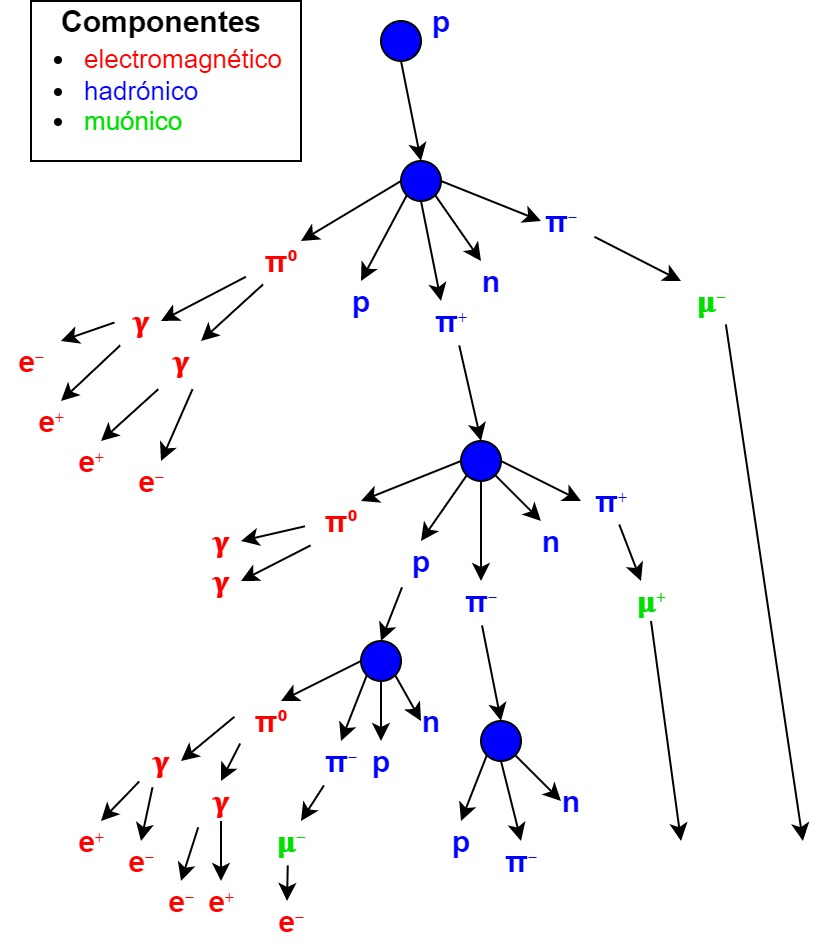
\includegraphics[width=50mm,scale=0.5]{Figures/showercomponents-jpg.jpg}
    \decoRule
    \caption[showercomponents]{caption figure 1}
    \label{fig:showercomponents}
\end{figure}

Los \textbf{rayos cósmicos} son partículas aceleradas en la galaxia o en objetos astrofísicos extragalácticos que al impactar con la atmósfera terrestre generan \textbf{cascadas de partículas} (Figura~\ref{fig:showercomponents}). El consenso general es que rayos cósmicos debajo de energías de 3x10e6 GeV son acelerados en los remanentes de supernovas galácticas y para energías mayores no se tiene una clara idea de que es lo que acelera a estas partículas, lo único que se tiene claro es de que dichas partículas tienen un orígen extragaláctico. A modo de comparación estas fuentes aceleran partículas en tres órdenes de magnitud mayor que el equivalente energético del LHC.

Cuando la energía de los rayos cósmicos sobrepasa significativamente 1000 GeV estos tienen que ser estudiados por las cascadas de partículas que generan en la atmósfera. La mayoría de las cascadas son iniciadas por hadrones con energías que van desde 1000  GeV o mayores a 10 TeV, que al entrar isotrópicamente a la atmósfera producen un gran número de productos secundarios en una serie de colisiones sucesivas con los núcleos de los constituyentes atmosféricos ie. N2, O2, Ar. Estos productos secundarios resultantes se comportan de una manera similar, mientras se van propagando a través de la atmósfera.

Las cascadas de partículas descritas anteriormente son conocidas como \textbf{cascadas atmosféricas extensas} \emph{EAS}. Estas cascadas atmosféricas se propagan longitudinalmente a lo largo de la dirección de incidencia de la partícula primaria, debido al momento transversal de los productos secundarios la cascada también se extiende lateralmente. Como referencia de la complejidad que se tiene, una partícula primaria altamente energética puede crear una cascada gigante de partículas que se propaga esencialmente a la velocidad de la luz a través de la atmósfera y puede alcanzar el nivel del mar si el evento es lo suficientemente energético agregado a lo anterior el número de productos secundarios es del orden 10e10 (Figura~\ref{fig:logitudinaldist}).

\begin{figure}
    \centering
    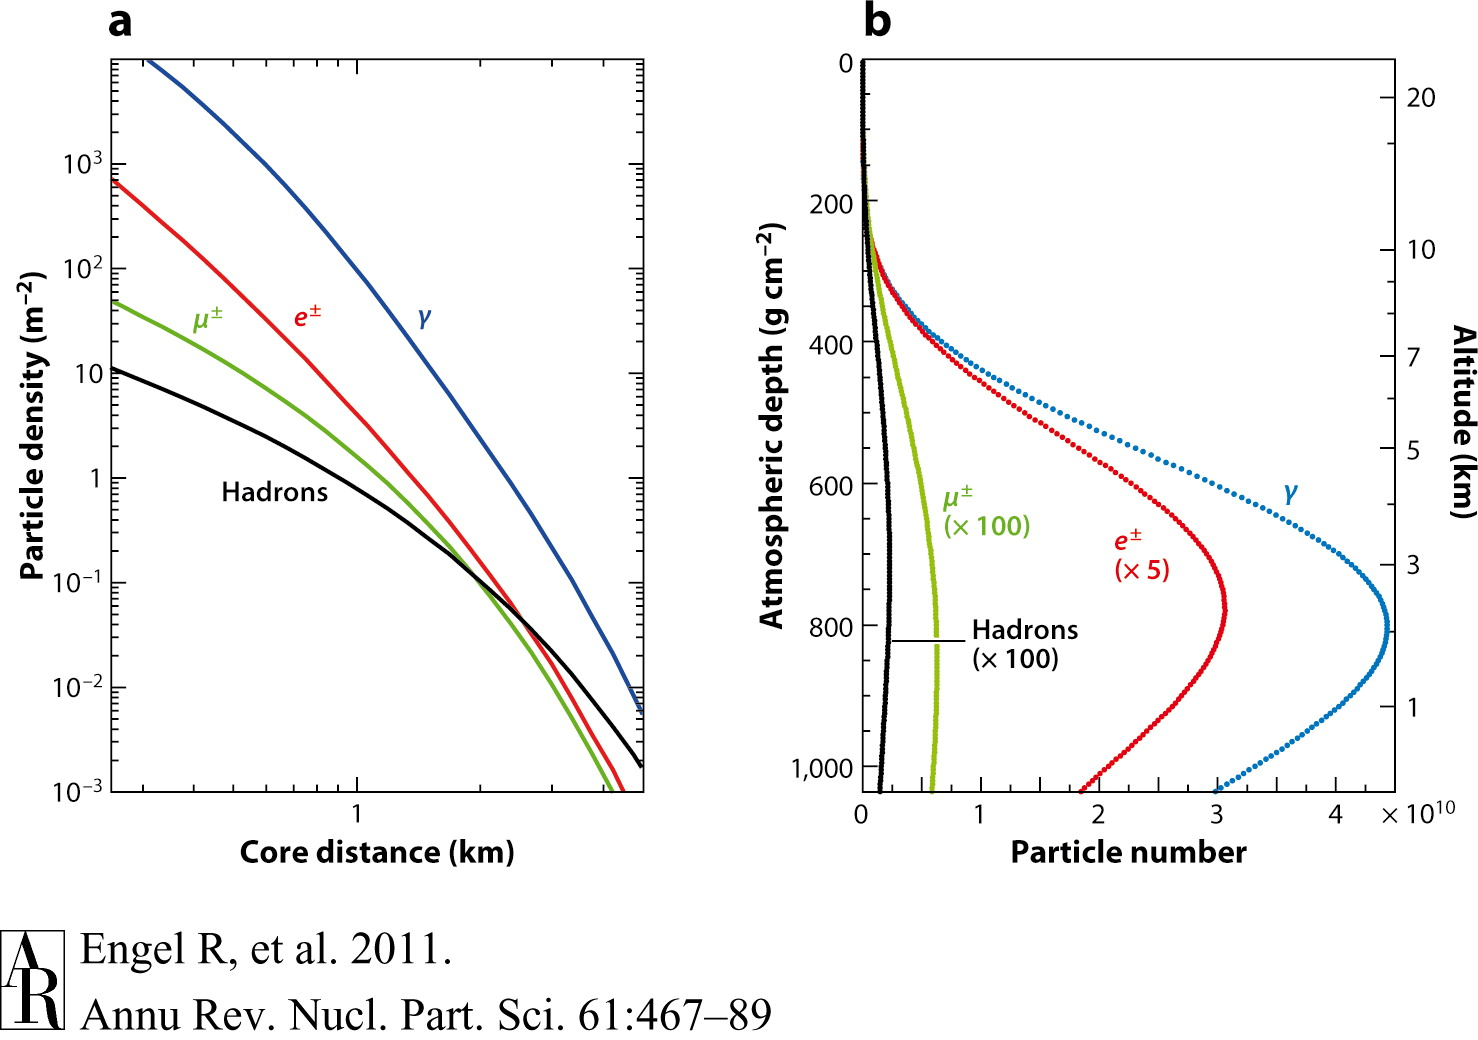
\includegraphics[width=50mm,scale=0.5]{Figures/logitudinaldistribution.jpeg}
    \decoRule
    \caption[logitudinaldist]{caption figure 1}
    \label{fig:logitudinaldist}
\end{figure}

\subsection{Propiedades de las cascadas atmosféricas}

Algunas propiedades que caracterizan a las cascadas atmosféricas son:

\begin{itemize}
    \item \textbf{E0} [eV]: energía de la partícula primaria. 
    \item \textbf{N} (\emph{shower size}): número total de partículas producidas en un nivel en particular de la atmósfera. Es una función que depende de la energía E0, ángulo de incidencia zenith angle y a altura de la primera interacción del evento primario en la atmósfera h1.
    \item \textbf{Xmax} [$gcm^-2$]: profundidad de máximo desarrollo medida desde la parte más alta de la atmósfera. Se desfasa a profundidades mayores conforme la energía del primario se incrementa.
    \item \textbf{Shower Axis}: extensión del vector de momento del primario incidente en la dirección de propagación de la cascada.
    \item \textbf{Dirección de arribo}: dirección de incidencia de la partícula primaria determinada por sus ángulos azimutales y el ángulo zenith.
\end{itemize}

\subsection{Métodos de detección}

Los principales detectores de cascadas atmosféricas son arreglos de detectores espaciados uno del otro en distancias que dependen de la energía de los rayos cósmicos que se quieren observar. Para energías de 10e6 GeV la distancia entre los detectores deben de ser del orden de decenas de metros y para energías que sobrepasan 10e9 GeV la distancia es del orden de miles de metros, por ejemplo en el observatorio Pierre Auger la distancia entre detectores es de 1500m. Diferentes métodos observacionales como detectores de aire cherenkov o detectores de fluorescencia son combinados con estos arreglos como en el caso del observatorio Pierre Auger (Figura~\ref{fig:eas}).

\begin{figure}
    \centering
    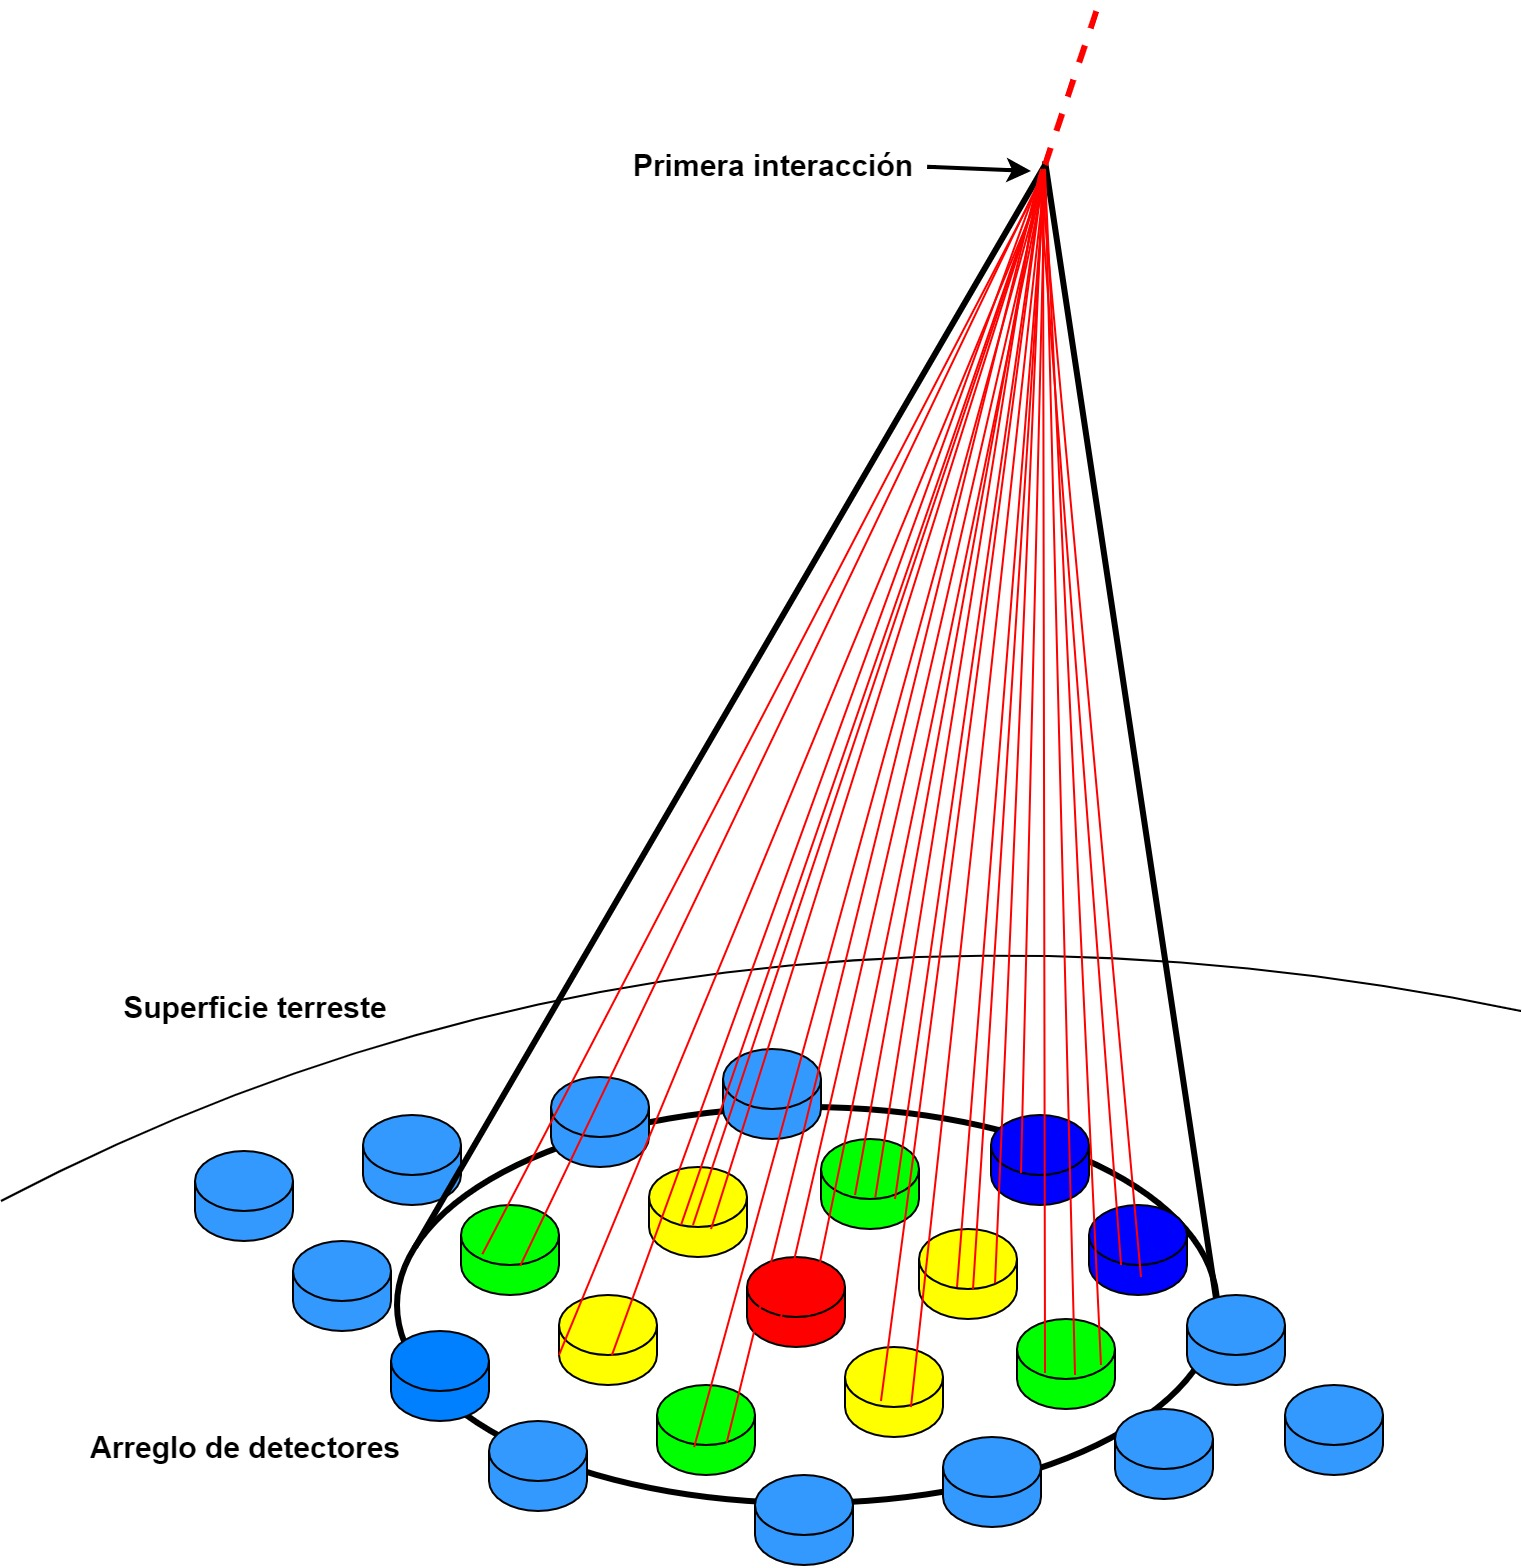
\includegraphics[width=50mm,scale=0.5]{Figures/eas-jpg.jpg}
    \decoRule
    \caption[eas]{caption figure 1}
    \label{fig:eas}
\end{figure}

Sin importar el tipo de sistema de detección que se use, los datos adquiridos representan a la cascada en una etapa en particular de su desarrollo, así como una foto instantánea de la cascada, en el plano de observación. Con estos datos se puede conocer información básica que caracteriza a la cascada atmosférica así como los tiempos de arribo de las partículas cargadas, fotones asociados no ópticos, las distribuciones laterales de partículas y fotones en el plano de observación a una profundidad atmosférica específica. Las propiedades anteriores son inmediatamente accesibles con un arreglo de detectores simple.

La reconstrucción de la partícula primaria depende del modelo hadrónico de interacciones que use el simulador Monte Carlo.

\section{Análisis de las cascadas atmosféricas}

Las cascadas atmosféricas están caracterizadas por un delgado disco de partículas radialmente extenso que se propaga a la velocidad de la luz a través del eje de la cascada. El patrón de las cascadas es circular para cascadas verticalmente incidentes, mientras que la extensión longitudinal y lateral dependen principalmente de la energía de la partícula primaria. El esparcimiento lateral de las partículas en regiones bajas de la atmósfera, llega a cubrir áreas de varios kilómetros cuadrados agregado a lo anterior la mayoría de las partículas arriban en intervalos estrechos de tiempo que van desde unos cuantos nanosegundos en la vecindad del eje de la cascada hasta unos 10 ns a distancias mayores del núcleo de la cascada.

Eventos de baja energía alcanzan su máximo desarrollo en zonas altas de la atmósfera y se mitigan lentamente a mayor profundidad; los componentes que alcanzan a llegar a la superficie son los muones y neutrinos. Para eventos extremadamente energéticos las cascadas logran alcanzar su máximo desarrollo a nivel del mar mientras que sus componentes hadrónicos y electromagnéticos sobrevivientes, son absorbidos en la superficie terrestre y los muones resultantes altamente energéticos continúan propagándose bajo tierra. 

Como regla de dedo se puede decir que en promedio una cascada atmosférica está constituida al $1\%$ por hadrones, alrededor del $10\%$ son muones y el $90\%$ o más son electrones o positrones. También para las primeras estimaciones energéticas de la primaria, se tiene que cascadas verticales a una altitud de 5km tienen una energía $~1$ GeV, $~3$ GeV para alturas entre 2.5 km y 3 km $~10$ GeV a nivel del mar.

\begin{figure}
    \centering
    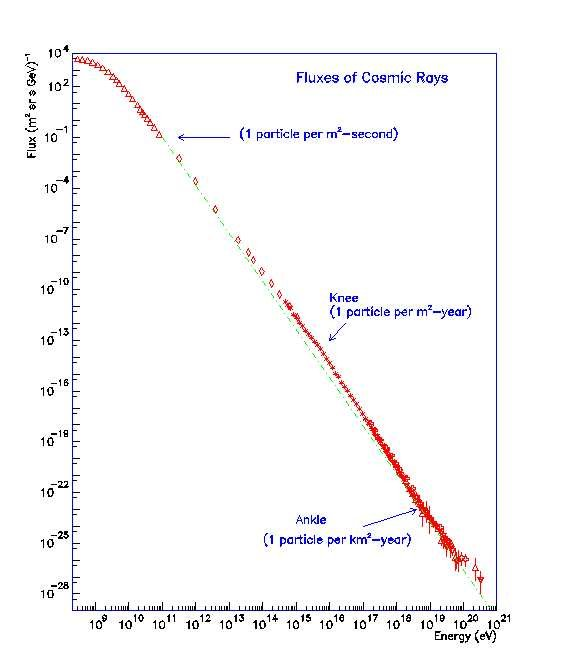
\includegraphics[width=50mm,scale=0.5]{Figures/All-particle-cosmic-rays-energy-spectrum.jpg}
    \decoRule
    \caption[energyspectrum]{caption figure 1}
    \label{fig:energyspectrum}
\end{figure}

Para poder visualizar la ocurrencia de estos eventos en distintos regímenes energéticos se puede estudiar el número de partículas que cruzan un área en un tiempo dado, conocido como flujo cósmico. Este flujo sigue una ley de potencias con la forma $\frac{1}{E^3}$, en se puede ver  energías alrededor de $10^12$ eV el flujo es de 10 partículas primarias por minuto y $m^2$, para energías entre $10^18$ eV y $10^19$ eV se tiene 1 partícula primaria por año y $km^2$ en estos regímenes energéticos las estadísticas son pobres y las incertidumbres altas. 

Los observables importantes que se deben de obtener para poder reconstruir una cascada son, el tiempo de arribo $t_i$ al detector $i$ respecto al tiempo de referencia $t_0$, la densidad de partículas $\rho_i$ y la posición del detector con respecto al sistema de referencia $(x_i, y_i)$.
Con la distribución lateral de las partículas su puede adquirir la localización del eje de la cascada y el tamaño de la cascada para así obtener un estimado de la energía. Los parámetros anteriores son clasificados como accesibles directamente ya que no necesitan un análisis complejo para su adquisición. 

Por último, parámetros indirectamente accesibles que se relacionan con la naturaleza de la partícula primaria, como el tipo de partícula, masa y carga, no se pueden extraer inmediatamente y requieren métodos sofisticados de análisis. 

La mayoría de las partículas arriban en intervalos estrechos de tiempo que van desde unos cuantos nanosegundos en la vecindad del eje de la cascada hasta unos 10 ns a distancias mayores del núcleo de la cascada.

\section{Simulaciones}

Simuladores de cascadas atmosféricas son de vital importancia para la evaluación e interpretación de datos experimentales. Las técnicas se reducen a crear e insertar un modelo de cascadas que corresponda a nuestro mejor entendimiento de la realidad, simular cascadas, comparar resultados con los datos experimentales, modificar el modelo o sus parámetros y intentar de nuevo; hacer ajustes pequeños al modelo y repetir hasta que se obtenga un consenso entre la predicción y el experimento.

Las cascadas iniciadas por primarios hadrónicos consisten en la superposición de dos tipos de cascadas, una hadrónica y otra electromagnética. La cascada electromagnética se entiende bien y solo posee problemas prácticos asociados al gran número de partículas participantes en el orden de $~10^10$. Los programas computacionales que simulan cascadas hadrónicas o electromagnéticas de alta energía o cascadas atmosféricas completas son altamente complejos.

Para tomar en cuenta la complejidad computacional que se tiene, una simulación completa de una cascada debe incluir los componentes electromagnéticos y hadrónicos. Además se debe de tomar en cuenta todos los procesos relevantes, donde la mayoría son de naturaleza estocástica y muchos están en competencia entre sí. También se debe incluir los parámetros que especifican el estado de cada partícula como su masa, carga, energía, momento, ubicación de su creación en el espacio tiempo x,y,z,t, la orientación angular respecto al marco de referencia y parámetros genéticos que revelan la altura de la interacción donde cada partícula fue creada. Estos observables son cruciales para análisis subsecuentes y para la comparación con datos experimentales.

\subsection{Estrategia para simulaciones de EAS}

La arquitectura del sistema ASICO sirve como base para entender el proceso de un simulador completo. ASICO fue el primer simulador que generaba cascadas detalladas al usar 12 parámetros que definen a cada partícula y este fue la base para el desarrollo de CORSIKA.
Para simular una cascada completa se comienza con la simulación de la cascada hadrónica y se le llama PASO 1, este paso da lugar a datos como la elasticidad, distribuciones de interacciones hadrónicas en diferentes rangos de energías, entre otros; para la parte electromagnética de la cascada se le llama PASO 2 y la combinación de las dos simulaciones para formar la cascada completa se le conoce como el PASO 3.

\begin{figure}
    \centering
    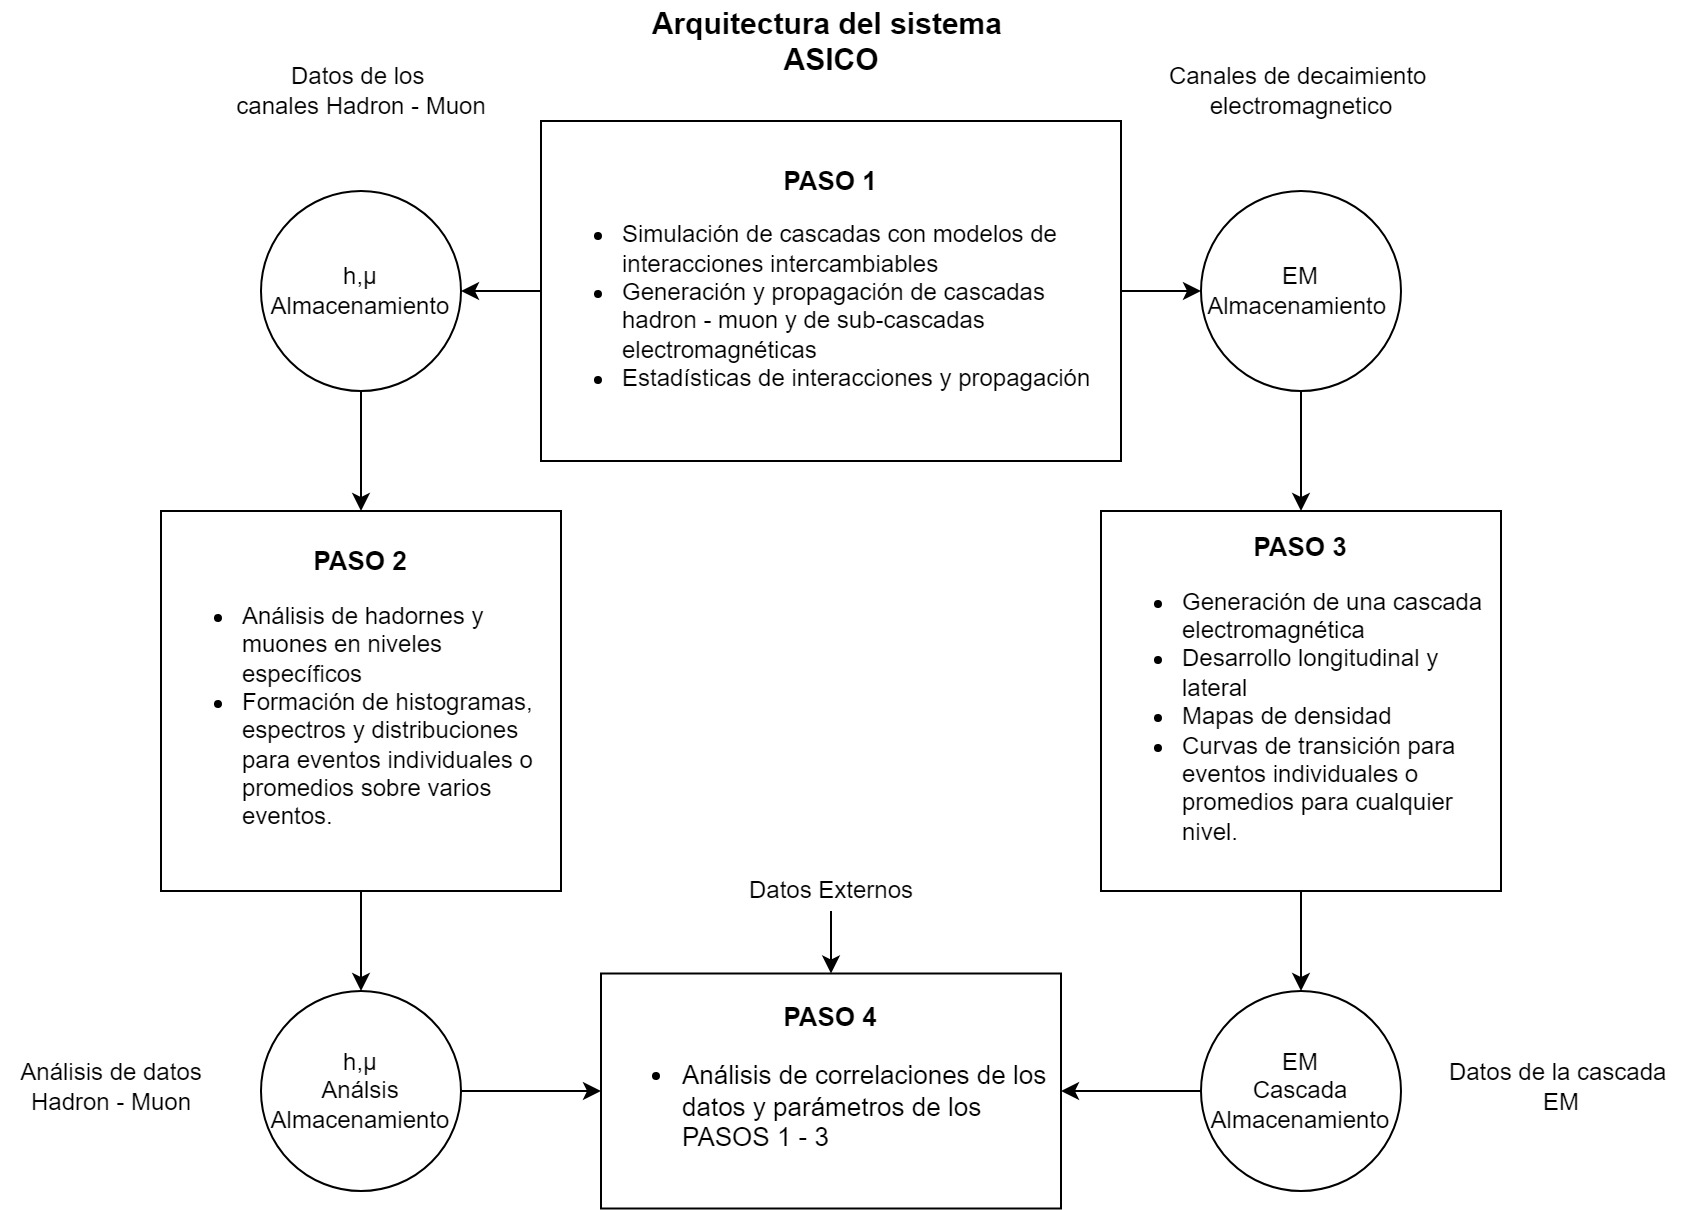
\includegraphics[width=50mm,scale=0.5]{Figures/asico-jpg.jpg}
    \decoRule
    \caption[asicoarq]{caption figure 1}
    \label{fig:asicoarq}
\end{figure}

% Hablar un poco más sobre cómo se usa Monte Carlo en los simuladores

\subsection{Problemática de las simulaciones}

Los parámetros que determinan a cada partícula se deben de asignar en su punto de creación y requieren actualizarse después de cada proceso al cual está sujeta. Esto es al final de cada trayectoria particular, después de propagarse al siguiente punto de interacción o decaimiento y cuando pasan a un nuevo nivel de observación. En cada actualización la partícula y sus parámetros son guardados para su subsecuente análisis y evaluación de los datos de la cascada simulada.

Consecuentemente, la ejecución de programas que simulan cascadas requieren mucho tiempo computacional  particularmente para cascadas energéticas donde el número de partículas involucradas se vuelve muy grande. La gran cantidad de datos producidos por estas simulaciones requieren también una gran capacidad de almacenamiento. La complejidad aumenta si los componentes atmosféricos cherenkov o de fluorescencia se incluyen, en este caso los datos corren el riesgo de divergir y métodos computacionales más sofisticados deben de ser usados para su análisis.

En general el desarrollo y la propagación de una cascada a partir del punto de iniciación (la primera interacción) hasta  el nivel de observación consume más tiempo que el análisis subsecuente de los datos producidos.

\begin{itemize}
    \item \textbf{Memoria:} Almacenamiento confiable de los datos crudos.
    \item \textbf{Rastreabilidad:} Rastreo de los parámetros que determinan a cada partícula.
    \item \textbf{Fenomenología:} Propagación de las partículas en la atmósfera tomando en cuenta todos los procesos a los que están sujetas.
    \item \textbf{Configuración inicial:} Correlación confiable entre los parámetros iniciales ( \emph{i.e.} modelos de interacción, propiedades del detector, propiedades de la primaria) con la cascada final
    \item \textbf{Tiempo:} Existe una relación lineal entre la energía de la partícula y el tiempo que lleva simular la cascada que genera.
\end{itemize}

\section{Modelos generativos}

Los modelos generativos son un tipo de aprendizaje no supervisado, que describen cómo se genera un conjunto de datos en términos de un modelo probabilístico. Al muestrear de dicho modelo se es capaz de generar datos no observados previamente. Típicamente el marco de trabajo de los modelos generativos involucra las siguientes partes.

\begin{itemize}
    \item \textbf{Los datos:} Conjunto de observaciones, que se asumen ser generadas de acuerdo a una distribución de probabilidad desconocida.
    \item \textbf{El modelo:} Un modelo generativo que intenta imitar lo mejor posible, a la distribución que genera las observaciones. Este modelo es capaz de generar datos no observados que parecen haber sido generados con la distribución desconocida y no debe de generar datos conocidos.
\end{itemize}

\subsection{Aplicación de modelos generativos}

Algunas de las tareas modernas de los modelos generativos son:

\begin{itemize}
    \item \textbf{Generación de datos novedosos:} Se generan datos nunca antes vistos que pueden ser utilizados para imitar fenómenos o para ayudar a flujos en modelos discriminativos con un pre entrenamiento autosupervisado.
    \item \textbf{Compresión de datos:} El modelo es capaz de aprender las características más importantes que determinan a la observación y así logra reducir la dimensionalidad del espacio de características donde vive la observación original. 
    \item \textbf{Tecnologías de síntesis condicional:} Proporciona un método capaz de generar información novedosa condicionada a un dominio específico. Lo anterior permite una suerte de transformación de datos de un dominio a otro. 
\end{itemize}

Las tareas anteriores han logrado avances en:

\begin{itemize}
    \item Generacion de rostros humanos
    \item Transformación de imágenes
    \item Transferencia de estilos
    \item Texto a imagen
    \item Texto a voz
    \item Edicion de imagenes
    \item Super resolución
    \item Generación de objetos 3D
    \item Predicción de fotogramas en videos
\end{itemize} 
%% Chapter Template

\chapter{Modelos generativos} % Main chapter title

\label{Chapter3} % Change X to a consecutive number; for referencing this chapter elsewhere, use \ref{ChapterX}

%----------------------------------------------------------------------------------------
%	SECTION 1
%----------------------------------------------------------------------------------------

Este capítulo proporciona una breve y concreta introducción a los modelos generativos, su fundamento teórico y algunas de las principales áreas de investigación. Además de mostrar las principales aplicaciones en HEP.

\section{Introducción}

Así como los modelos discriminativos han sido el centro del progreso en metodologías del aprendizaje máquina en los últimos años ya que es más sencillo monitorear su desempeño y así poder elegir la mejor metodología que se ajuste a la tarea. Los modelos generativos suelen ser más difíciles de evaluar, lo cual hace que encontrar aplicaciones industriales sea más complicado. 

Los modelos generativos han probado su efectividad para generar muestras que son capaces de imitar a observaciones reales así como rostros humanos con StyleGAN de NVIDIA o GPT3 de openAI para generar texto. Los modelos anteriores han impulsado el interés para expandir el campo del aprendizaje de máquina a través de modelos que aprenden a generar muestras indistinguibles de observaciones reales. Los avances en el campo podrían ser fundamentales para el desarrollo de una máquina que haya adquirido una inteligencia comparable a la de los humanos.

El campo de los modelos generativos es diverso y la definición de los problemas toman una gran variedad de formas. Sin embargo, para cada tarea, los desafíos que se tienen son los mismos. Entender cómo  es que el modelo maneja un alto grado de dependencias condicionales entre las características de la observación y como es que logra encontrar una observación viable, en un espacio de alta dimensionalidad, que concuerda con los datos observados a partir de un conjunto pequeño de observaciones, es de vital importancia para desarrollar metodologías más robustas.

\subsection{Fundamento teórico}

Como punto de partida se debe de reconocer la diferencia clave entre los modelos discriminativos y los modelos generativos. 

Def.

Los modelos discriminativos estiman p(y|x) - la probabilidad del observable y dada la observación x.

Los modelos generativos estiman p(x) - la probabilidad de observar x.

En otras palabras, los modelos discriminativos intentan estimar la probabilidad de que una observación x pertenezca a la categoría y, y los modelos generativos intentan estimar la probabilidad de ver la observación x. Por lo tanto el modelo debe de ser probabilístico en vez de ser determinista y debe incluir un elemento estocástico que influencia las observaciones individuales generadas por el modelo.

\section{Líneas de investigación}

Detrás del creciente interés en la academia por los modelos generativos se encuentran dos razones con una gran importancia teórica, que se describen a continuación:

Se debe de buscar un entendimiento completo de cómo se generan las observaciones para así poder formar inteligencias artificiales más sofisticadas que van más allá de lo que pueden lograr los modelos discriminativos. 

Es altamente probable que los modelos generativos sean centrales para futuros desarrollos  en otros campos del aprendizaje máquina.

\section{Modelos generativos}

Un modelo generativo describe cómo se genera un conjunto de observaciones en términos de un modelo probabilístico. Al generar muestras de este modelo, se es capaz de generar observaciones nunca antes vistas. 

Al tener un conjunto de observaciones que representen la entidad que se quiere generar. El objetivo del modelo generativo es generar nuevas observaciones que sigan las mismas reglas con las cuales las observaciones originales fueron generadas. Lo anterior es posible debido a que se asume que existe alguna distribución de probabilidad que explica, porqué ciertas observaciones son más probables de encontrarse en un conjunto y otras no. 

El trabajo del modelo es imitar una distribución desconocida lo más cercano posible, para luego muestrear de ella y generar nuevas observaciones, distintas de las conocidas, que además parezca que son parte del conjunto de entrenamiento.

El marco de trabajo de los modelos generativos es el siguiente:

1 Se tiene un conjunto de datos de observaciones $X$.

2 Se asume que las observaciones $X$ se generaron de acuerdo a una distribución de probabilidad desconocida $p_{datos}$.

3 Se diseña un modelo generativo $p_{modelo}$ que intenta imitar a $p_{datos}$.

4 Se muestrea de $p_{modelo}$ para generar observaciones que parecen ser obtenidas de $p_{datos}$.

Consideramos que $p_{modelo}$ hace un buen trabajo si:

Puede generar observaciones que parecen ser obtenidas de $p_{datos}$.

Puede generar observaciones que son sustancialmente diferentes a las observadas en X. En otras palabras, el modelo no debería de reproducir cosas que ya conoce.

\subsection{Conceptos básicos}

Def:

Espacio Muestral

El espacio muestral es el conjunto de todos los posibles valores que una observación x puede tomar.

Función de densidad de probabilidad

Una función de densidad de probabilidad, $p(x)$, es una función que mapea un punto x del espacio muestral a un número entre 0 y 1. La suma de la función de densidad sobre todos los puntos del espacio muestral es igual a 1 para que sea una distribución bien definida.

Por definición tenemos que solo existe una $p_{datos}$ pero existen infinitas distribuciones $p_{modelo}$ que pueden estimar $p_{datos}$. Para encontrar una distribución adecuada se tiene que usar un modelo paramétrico.

Modelo paramétrico

Un modelo paramétrico, $p_{\theta}(x)$, es una familia de funciones de densidad que pueden ser descritas por medio de un número finito de parámetros, $\theta$.

%% Chapter Template

\chapter{Método experimental} % Main chapter title

\label{Chapter4} % Change X to a consecutive number; for referencing this chapter elsewhere, use \ref{ChapterX}

%----------------------------------------------------------------------------------------
%	SECTION 1
%----------------------------------------------------------------------------------------
En este capítulo se detallan las técnicas utilizadas así como el método experimental para la generación y evaluación de cascadas atmosféricas.. 

\section{Recolección y manejo de datos}

Dado que el objetivo de este trabajo es implementar un modelo generativo que sea capaz generar simulaciones de cascadas atmosféricas, se necesita un banco de datos de dichas simulaciones. Una de las primeras maneras de obtener este conjunto de datos será tomar el simulador CORSIKA y generar el número de eventos necesarios para poder entrenar a la red neuronal. Como segunda opción de recolección se buscará un banco de simulaciones disponibles al público con características fundamentales como la energía de la primaria, la altura de máximo desarrollo, etc.

Como se ha mencionado en capítulos anteriores, las tareas que cada simulador conlleva para generar una cascada, incluyen subrutinas se encargan de la parte hadrónica, la parte electromagnética, el modelo de interacción, el rastreo de parámetros y procesamientos adicionales para reducir la carga computacional; por lo cual los datos que se utilizaran no deben de concentrarse en alguna de estas subrutinas para poder acotar el dominio de la simulación. 

%El análisis de simulaciones de cascadas se hace con procesamientos para obtener las distribuciones longitudinales de la cascada …

Para generar un resultado significativo sin pérdida de generalidad, se tomarán en cuenta las siguientes consideraciones:

Utilizar un número relativamente “grande” de simulaciones.
El número de observaciones debe ser un número “grande”, como referencia se intentará obtener un conjunto de datos con al menos el mismo número de observaciones que el conjunto MNIST.  

Preprocesar el conjunto de datos.
Para datos como los tiempos de arribo, el dominio de cada simulación diferirá en magnitudes que deben de tomarse en cuenta, por lo tanto técnicas de estandarización podrán ser utilizadas para tener una mejor estabilidad al entrenar el modelo. 

Separación en conjuntos de entrenamiento, validación y evaluación. 
Una vez que se cumpla lo anterior, los datos estarán listos para poder entrenar al modelo.

\section{Algoritmos}

\begin{algorithm}
    \caption{Algoritmo de entrenamiento de la GAN}\label{alg:cap}
    \begin{algorithmic}
    \Require $k \geq 1$
    % \Require $y = x^n$
    \For {$N$ iteraciones}
        
    \EndFor
    \State $y \gets 1$
    \State $X \gets x$
    \State $N \gets n$
    \While{$N \neq 0$}
    \If{$N$ is even}
        \State $X \gets X \times X$
        \State $N \gets \frac{N}{2}$  \Comment{This is a comment}
    \ElsIf{$N$ is odd}
        \State $y \gets y \times X$
        \State $N \gets N - 1$
    \EndIf
    \EndWhile
    \end{algorithmic}
\end{algorithm}

\section{Desarrollo del método}

A continuación se muestra el método desglosado. 
Obtener un banco de datos de simulaciones de cascadas atmosféricas acotadas a algún proceso seleccionado.

Hacer el preprocesamiento de datos adecuado para normalizar la entrada de datos y así estabilizar el entrenamiento sin dejar de tomar en cuenta las consideraciones teóricas que dicho procesamiento implica.

Elegir una arquitectura generativa adversaria y entrenarla para intentar generar nuevas cascadas.

Se tomarán las nuevas muestras y se inspeccionarán visualmente comparándolas con las observaciones originales.

Después de haber confirmado la similitud con las observaciones originales, se hará un análisis exploratorio de la dimensionalidad del vector latente y un análisis al proceso determinista de entradas y salidas de dicha red. 

Una vez logrado lo anterior, cambiar de arquitectura y repetir el proceso, si se puede.

\subsection{Mapa del método experimental} 
%% Chapter Template

\chapter{Resultados} % Main chapter title

\label{Chapter5} % Change X to a consecutive number; for referencing this chapter elsewhere, use \ref{ChapterX}

%----------------------------------------------------------------------------------------
%	SECTION 1
%----------------------------------------------------------------------------------------

Este capítulo muestra algunos de los resultados obtenidos por el método experimental presentado en el capítulo anterior.

\section{Discusión de resultados obtenidos}

A continuación se describirán los resultados por cada etapa del método experimental.

\subsection*{Obtención de datos y procesamiento}

Para obtener el conjunto de datos, primero se optó por intentar generar una base de datos usando el simulador CORSIKA, sin embargo, se observo que la generación de un dataset de al menos $60000$ observaciones, tomaría un tiempo inviable con el equipo de cómputo con el que se disponía. Del mismo modo, la complejidad adicional que la interfaz del programa y la inexperiencia con el mismo, agregaba una dificultad extra a la hora de configurar los parámetros del evento. 

Por consiguiente, se decidió buscar una base de datos de simulaciones que estuvieran disponibles al público. De modo que el banco de datos que se usó fue tomado de \parencite{Erdmann2018b}, el cual contiene $100000$ simulaciones de cascadas electromagnéticas con los siguientes parámetros.

%insertar tabla de df.info()

Para la selección y preprocesamiento de datos se seleccionó la señal que contiene los tiempos de arribo y la energía asociada a cada cascada. Después se hizo el ajuste propuesto en \parencite{Erdmann2018b} a los tiempos de arribo \ref{eq:}, sin embargo el ajuste no lograba estandarizar los datos, así que se hizo un mapeo lineal al dominio $[-1,1]$.

%insertar ajuste propuesto
%insertar imagenes post procesamiento y pre procesamiento

Para el escalar de la energía de cada cascada, se decidió categorizar la variable continua en $4$ rangos energéticos, los cuales son $x$.

%insertar tabla de post procesamiento y pre procesamiento

\subsection*{Modelo y entrenamientos}

Para la arquitectura del modelo se optaron por capas convolucionales para preservar la información entre detectores y los modelos tienen las siguientes propiedades.

%insertar info de los modelos en un tabla
El único parámetro que se modificó fue la dimensión del vector latente, y se guardaron los modelos resultantes para cada dimensión, sin embargo se observó que para dimensiones bajas el modelo llegaba a un colapso de modos con más frecuencia, como se muestra a continuación. 

%insertar tabla de modelos dimension vector latente y mode collapse
%insertar gráficas de pérdidas en el entrenamiento.

\subsection*{Generación de cascadas electromagnéticas}

Cascadas electromagnéticas generadas con los modelos 
%\ref{tabla}

%insertar cascadas generadas.

Comparación con las cascadas de entrenamiento.

Comparación con $50$ cascadas generadas usando CORSIKA.

\subsection*{Combinaciones lineales de vectores latentes}

Resultados al promediar vectores latentes y hacer una combinación lineal de estos para después ser insertados en categorías energéticas diferentes.

%insertar imágenes.

\begin{table}
    \caption{The effects of treatments X and Y on the four groups studied.}
    \label{tab:treatments}
    \centering
    \begin{tabular}{l l l}
        \toprule
        \textbf{Groups} & \textbf{Treatment X} & \textbf{Treatment Y} \\
        \midrule
        1 & 0.2 & 0.8\\
        2 & 0.17 & 0.7\\
        3 & 0.24 & 0.75\\
        4 & 0.68 & 0.3\\
        \bottomrule\\
    \end{tabular}
\end{table}

(e.g. Table~\ref{tab:treatments}).


\lstinputlisting[language=Python]{Code/dfa.py}
 

%----------------------------------------------------------------------------------------
%	THESIS CONTENT - APPENDICES
%----------------------------------------------------------------------------------------

\appendix % Cue to tell LaTeX that the following "chapters" are Appendices

% Include the appendices of the thesis as separate files from the Appendices folder
% Uncomment the lines as you write the Appendices

% Appendix A

\chapter{Arquitecturas} % Main appendix title

\label{AppendixA} % For referencing this appendix elsewhere, use \ref{AppendixA}

\section{Descripción de las capas}

La información de las capas de generador se encuentra en la tabla \ref{tab:GenArq}. Para un vector latente de dimensión $4$ se tienen $1053329$ parámetros de los cuales todos son parámetros de entrenamiento. Y para el modelo discriminador en la tabla \ref{tab:DiscArq}. Este modelo tiene un total de $1111365$ parámetros.

\begin{table*}
    \caption{Capas del generador $G_\theta$}
    \label{tab:GenArq}
    \centering
    \begin{tabular}{l l l}
        \hline
        \textbf{LayerName} & \textbf{Size} & \textbf{Nparams} \\
        \hline
        gen\_net.0.0.weight & 	 (8, 256, 3, 3)& 	 18432\\
        gen\_net.0.1.weight & 	 (256,)& 	 256\\
        gen\_net.0.1.bias & 	 (256,)& 	 256\\
        gen\_net.0.1.running\_mean & 	 (256,)& 	 256\\
        gen\_net.0.1.running\_var & 	 (256,)& 	 256\\
        gen\_net.0.1.num\_batches\_tracked & 	 ()& 	 1\\
        gen\_net.1.0.weight & 	 (256, 256, 3, 3)& 	 589824\\
        gen\_net.1.1.weight & 	 (256,)& 	 256\\
        gen\_net.1.1.bias & 	 (256,)& 	 256\\
        gen\_net.1.1.running\_mean & 	 (256,)& 	 256\\
        gen\_net.1.1.running\_var & 	 (256,)& 	 256\\
        gen\_net.1.1.num\_batches\_tracked & 	 ()& 	 1\\
        gen\_net.2.0.weight & 	 (256, 128, 3, 3)& 	 294912\\
        gen\_net.2.1.weight & 	 (128,)& 	 128\\
        gen\_net.2.1.bias & 	 (128,)& 	 128\\
        gen\_net.2.1.running\_mean & 	 (128,)& 	 128\\
        gen\_net.2.1.running\_var & 	 (128,)& 	 128\\
        gen\_net.2.1.num\_batches\_tracked & 	 ()& 	 1\\
        gen\_net.3.0.weight & 	 (128, 128, 3, 3)& 	 147456\\
        gen\_net.3.1.weight & 	 (128,)& 	 128\\
        gen\_net.3.1.bias & 	 (128,)& 	 128\\
        gen\_net.3.1.running\_mean & 	 (128,)& 	 128\\
        gen\_net.3.1.running\_var & 	 (128,)& 	 128\\
        gen\_net.3.1.num\_batches\_tracked & 	 ()& 	 1\\
        gen\_net.4.weight & 	 (128, 1, 3, 3)& 	 1152\\
        gen\_net.4.bias & 	 (1,)& 	 1\\
        embed.weight & 	 (4, 4)& 	 16\\
        \hline
    \end{tabular}
\end{table*}

\begin{table*}
    \caption{Capas del Discriminador $D_\phi$}
    \label{tab:DiscArq}
    \centering
    \begin{tabular}{l l l}
        \hline
        \textbf{LayerName} & \textbf{Size} & \textbf{Nparams} \\
        \hline
        critic\_net.0.0.weight& 	 (64, 2, 3, 3)& 	 1152\\
        critic\_net.0.1.weight& 	 (64,)& 	 64\\
        critic\_net.0.1.bias& 	 (64,)& 	 64\\
        critic\_net.1.0.weight& 	 (128, 64, 3, 3)& 	 73728\\
        critic\_net.1.1.weight& 	 (128,)& 	 128\\
        critic\_net.1.1.bias& 	 (128,)& 	 128\\
        critic\_net.2.0.weight& 	 (128, 128, 3, 3)& 	 147456\\
        critic\_net.2.1.weight& 	 (128,)& 	 128\\
        critic\_net.2.1.bias& 	 (128,)& 	 128\\
        critic\_net.3.0.weight& 	 (256, 128, 3, 3)& 	 294912\\
        critic\_net.3.1.weight& 	 (256,)& 	 256\\
        critic\_net.3.1.bias& 	 (256,)& 	 256\\
        critic\_net.4.0.weight& 	 (256, 256, 3, 3)& 	 589824\\
        critic\_net.4.1.weight& 	 (256,)& 	 256\\
        critic\_net.4.1.bias& 	 (256,)& 	 256\\
        critic\_net.5.weight& 	 (1, 256, 3, 3)& 	 2304\\
        critic\_net.5.bias& 	 (1,)& 	 1\\
        embed.weight& 	 (4, 81)& 	 324\\
        \hline
    \end{tabular}
\end{table*}
%\include{Appendices/AppendixB}
%\include{Appendices/AppendixC}

%----------------------------------------------------------------------------------------
%	BIBLIOGRAPHY
%----------------------------------------------------------------------------------------

\printbibliography[heading=bibintoc]

%----------------------------------------------------------------------------------------

\end{document}  
